


\section{Final Product}
- detailed description about how the client and server app look like and how it works.

\subsection{Server-side application}

Maybe we can present milestones reached

\begin{figure}[H]
	\centering
		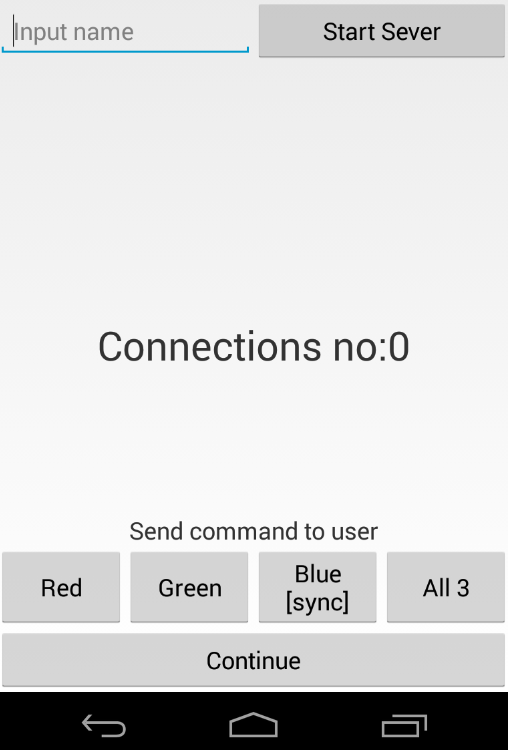
\includegraphics[width=5cm]{conclusion/server_ui.png}
	\caption{Server UI}
	\label{fig:Server_UI }
\end{figure}

\subsection{Client-side application}
\begin{figure}[H]
	\centering
		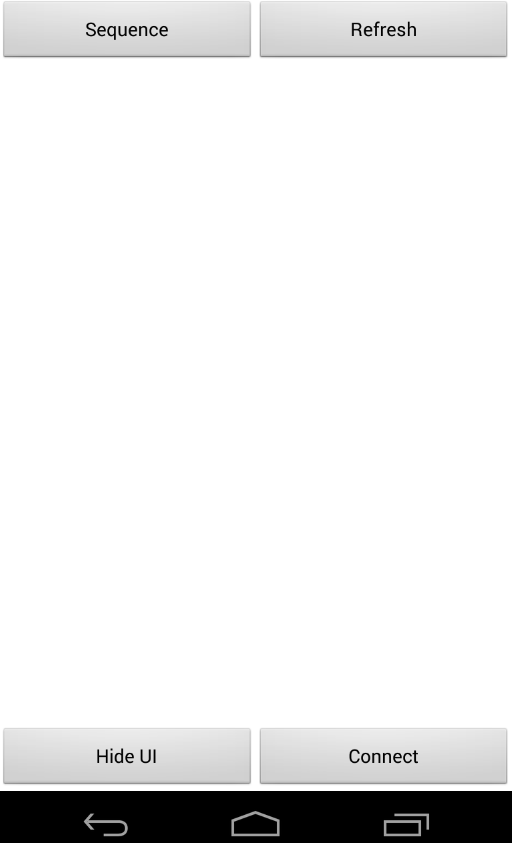
\includegraphics[width=7cm]{conclusion/user_ui.png}
	\caption{Client UI}
	\label{fig:Client_UI }
\end{figure}

\subsection{Functionalities}
???
%\section{Evaluation criteria}
%\section{Evaluation Results}
%\section{Conclusion}
%\section{Discussion}
\section{Further work}

One of the main challenges for future is to improve the performance.
Higher FPS\footnote{Frames Per Second} value would allow to display more interesting animations or even videos.
Also scalability in sense of number of client devices should be improved.

%___ DEVICE TRACKING ________________
One of the first steps in further development is \emph{device tracking}.
Once the mobile device is detected, its position is saved but not updated during time.
It is probable, that on rock concerts, the audience wont be static, but it will be in motion.
The current product would not be able to deal with that situation and the content would not be displayed properly.
One of the solutions might be to perform the initial detection and during playing the media it is known what color should each mobile device display and therefore the playing could be considered as a another continuous detection of devices.

%___ GRID ADJUSTING ________________
Further work can also be focused on \emph{grid adjusting}.
In non-artificial situations, it is possible, that the audience will be located only in the edge of the camera's snapshot.
The current prototype would not adjust to that situation, although it would be desired.
It would be adequate to keep the grid's dimension but to adjust the its resolution and position it to the edge, where audience is located.
One of the benefits of this extension is that the person who is controlling device with camera would not have to position and zoom it precisely.

%___ IMPROVE IMAGE PROCESSING  ________________
Even though device detection worked fine in dark environment, there are fields in which it could be improved.
The tree algorithm, described in Section \ref{subsec:tree_alg} will not work properly, when more devices are in the same tile.
Although there is a fallback algorithm, which will succeed in this case, its time complexity is too high for large audience.
Hence, a new algorithm with similar performance as the tree algorithm is desired.
Last but not least, if the detection works even in worse light conditions it would significantly grow the potential of the product.

%___ SCREEN NOT PIXEL ________________
One of the interesting ideas for extension is not to display single color on a client device, which therefore works as a one pixel, but to display several pixels or even part of an image.
It would be possible to display complex images or videos even on few devices as can be seen in Figure \ref{fig:extension}.
This concept would required not only detection of position of devices but also finding its orientation.


\section{Summary}
During this project the "blablabla" was designed. ...


- reflect non nonfunctional requirements